\begin{frame}
    \frametitle{Estimates from the negative binomial model}
	With estimates for $\eta_1$, $\alpha$, and $\gamma$, we can use (\ref{eq:deltaAG}) to estimate the number of new words we would see in $tS$ ``more'' Shakespeare.
	\medskip
	
	For $\hat\eta_1$ we used the unbiased estimate $n_1$, and for $\alpha$ and $\gamma$ we used the observed data for the first $x_0$ frequency counts, $x_0=5, 10, 15, 20, 30,$ and~$40$ to calculate maximum likelihood estimates from the NB model.
	\pause
	
	Here is what we got:
	\vspace*{-5mm}
	\begin{center}
		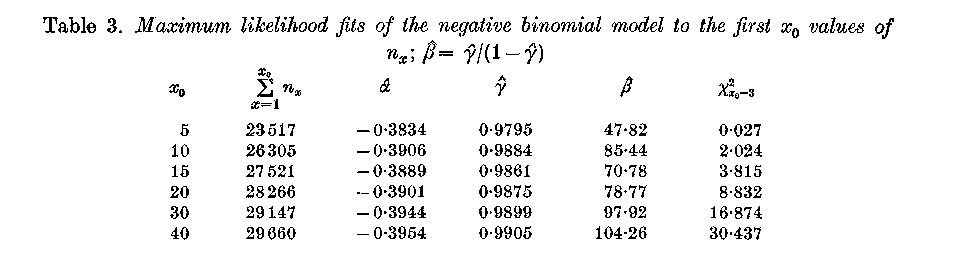
\includegraphics[width=4.5in]{../compendium/Figures/ET-Table3.pdf}
	\end{center}
	\pause	
	{\color{red} Can Table~3 be reproduced?}
\end{frame}
